\chapter{Literature Review}

This chapter will provide a review of the existing literature, which will be used guide the student in their planning and development efforts of the project.

\noindent As such, it will be covering the following areas:
\begin{itemize}
    \item Software development methodologies
    \item Requirement gathering
    \item Tech stack
    \item Large Language Models (LLMs)
    \item Gap Analysis
\end{itemize}

\section{Software development methodologies}

\subsection{Software Development Life Cycle}

The Software Development Life Cycle (SDLC) is a process used to guide the development of software applications or systems \parencite{sdlc1}. The SDLC consists of multiple phases, each with its own set of activities and deliverables. \textcite{sdlc2} outline the phases of the SDLC as following:
\begin{enumerate}
    \item Requirement gathering and analysis phase - the requirements are gathered from the project stakeholders and saved in a specific document. Based on the requirements gathered, a development plan is created and a feasibility study is conducted.
    \item Design phase - the previously gathered requirements are written in a more technical manner and system deisngs are created that will later guide the developers to develop the software. 
    \item Implementation phase - Actual development of the software occurs in this phase. Additionally, some smaller unit tests may be done during this phase as parts of the software are developed.
    \item Testing phase - may involve multiple types of testing, such as unit testing, integration testing, and system testing. \textcite{testing} describes the different types of tests as following:
    \begin{itemize}
    \item Unit testing - done on the lowest level of the software, testing individual units or components of the software.
    \item Integration testing - performed on two or more units combined together, usually focusing on the interfaces between these components.
    \item System testing - focuses on the `end-to-end quality of the entire system', testing it as a whole based on the system requirement specification.
    \end{itemize}
    \item Maintenance phase - involves the deployment and maintenance of the software. Additionally, this phase may include user acceptance testing, where the software is handed over to the end-users to ensure that it meets their needs \parencite{testing}. 
\end{enumerate}

\begin{figure}[ht]
    \centering
    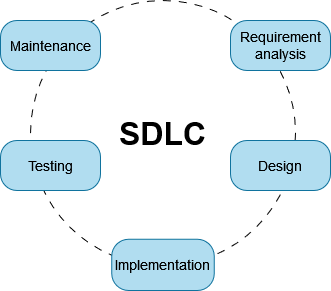
\includegraphics[scale=0.6]{SDLC.png}
    \caption{Software Development Life Cycle}
    \label{fig:sdlc}
\end{figure}

\newpage

\subsection{SDLC Models}

The literature describes several SDLC models that have been used in the development of software applications. \textcite{sdlc1, sdlc2} outline the most common SDLC models:
\begin{itemize}
    \item Waterfall Model
    \item V Model
    \item Spiral Model
    \item Iterative Model
    \item Agile model
\end{itemize}

Due to the nature of the project being different to traditional software development projects, and the student's familiarity with only Waterfall and Agile models, the next sections will only focus on these two models.

\subsubsection{Waterfall Model}

The Waterfall Model is the most well-known SDLC model. It is a linear model, where the development process is divided into distinct, sequential phases that follow the SDLC.

The Waterfall Model's strengths lie in its simplicty of use, ease of understanding and a structured approach \parencite{waterfall}. An additional stregth of the Waterfall model that the authors note is its extensive documentation and planning, which is done in the early stages of a project, that is also maintened throughout the project. These two factors also help minimize the overhead that comes with planning and management of a project.

One of its main weaknesses, mentioned by \textcite{waterfall}, is its lack of flexibility in regards to change of requirements. As such, once the project leaves the requirements analysis or design phase, it may be difficult to make any changes to the project deliverable. Thus, this model is not suitable for projects where the requirements are not well understood or are likely to change. Finally, the deliverable is only available at the end of the project, so the end-users can provide any feedback during its development \parencite{waterfall}.

% Add a figure maybe?

\subsubsection{Agile Model}

Another well-known model is Agile. It focuses on the idea that requirements are not always well-known and accepting that change is inevitable \parencite{agile}. Similarly, as the author mentions, the focus of this methodology is on continuous delivery of software and interaction with the customer to get feedback. The author mentions that Agile is well known for its flexibility and adaptability to change, its ability to deliver working software in short iterations and its focus on customer satisfaction.

Agile has multiple frameworks that can be used to guide the development process, such as Scrum or Kanban. Scrum is an Agile framework, where the project is divided into sprints, each lasting between 2-4 weeks and focusing on delivering value to the customer through incremental software features \parencite{scrumban, agile}. On the other hand, Kanban focuses on visualizing the project workflow through a visual board by using columns, cards and swimlanes. Kanban's main goal is to limit the work in progress through column limits and a pull system to maximize the flow of work through the system \parencite{agile}.

Agile does have some drawbacks - its lack of documentation and formal planning, especially in the early stages of the project, may not be suitable for large scale projects, where extensive documentation and planning are required \parencite{sdlc1, agile, sdlc2}. Similarly, the Agile model may not be suitable for projects where the requirements are well understood or where there may be strict regulations that guide how the project should be developed.

Nowadays, the use of Scrum and Kanban together is becoming quite popular, with many teams employing both frameworks in their projects. As \textcite{scrumban} mention, this can be quite beneficial as it allows teams to adopt the appropriate practices of both methods and adapt them accordingly based on their needs.

% Add some figures for Scrum and Kanban

\subsection{A hybrid approach}

For many years, Waterfall has been the most widely used model in software development projects, with Agile approaches gaining popularity in the recent years \parencite{hybrid1}. However, a hybrid approach has also been emerging, with various surveys reporting a combined approach being used in project work \parencite{hybrid1,hybrid2}. The most common combinations that form this hybrid approach are Scrum, Iterative Development, Kanban, Waterfall and DevOps, with the approach that combines Waterfall and Scrum being the most popular \parencite{hybrid2}. In that case, only the development part is usually done in an Agile way - with the rest of the project using the traditional approach as a backbone \parencite{hybrid2}.

\textcite{hybrid1} note that projects using either Agile, traditional or hybrid approach show similar levels of success in terms of budget, time and quality. However, the authors have found that agile and hybrid approaches perform much better on the customer satisfaction metric than the traditional counterpart.

\section{Requirements gathering}

Regardless of the approaach used, the requirements gathering phase is the first step in any software development process. As described by \textcite{reqanalysis2}, a requirement is a `necessary attribute in a system\ldots that identifies a capability, characteristic, or quality factor of a system in order for it to have value and utility to a user'. Multiple studies mention how proper requirement gathering plays a pivotal role in the project quality and success, with a majority of project failures being attributed to poor requirements gathering \parencite{reqanalysis1, reqanalysis3, reqanalysis5}.

\subsection{Requirement types}

Requirements can be classified into 2 categories: functional and non-functional requirements. Functional requirements describe the system's behavior, such as what the system should do and how it will react to different inputs, while non-functional requirements describe the system's quality attributes, such as performance, security, reliability, etc. \parencite[6]{requirements}.

When writing the requirements in a document, it is important to ensure that everything is written in a clear and concise manner to avoid any ambiguity. As such, \textcite[112]{requirements} recommends using a standard format for writing all requirements: using simple language in a consistent manner, avoiding the use of technical jargon, vague terms and not creating multiple requirements in a single statement.

Similar principles of writing requirements can be found in \textcite{requirements2} which also provides a list of requirement characteristics: necessary, appropriate, unambiguous, complete, singular, feasible and verifiable. The same standard recommends using attributes to describe each requirement, such as an identification, owner, priority, risk, rationale, difficulty, and type (functional/non-functional).

Prioritizing requirements is another crucial task, especially in projects with numerous requirements. Some methods include using a low to high priority, assigning a numerical value within a specific range or MoSCoW, which classifies requirements into four categories: 
\begin{itemize}
    \item Must have - must be implemented in the software before being released
    \item Should have - important but not necessary for the software to be released
    \item Could have - desirable but not necessary for the software to be released
    \item Won't have - requirements that are not included in the current release
\end{itemize}

\subsubsection{Requirements in Agile}

In Agile projects, the most basic unit of requirements are usually written in the form of User Stories, which are simple descriptions of a feature desired by the customer \parencite[191]{requirements}. User Stories are written in a specific format, such as `As a [user], I want to [action] so that [benefit]'. Other components of a User Story include a title, acceptance criteria (conditions that must be met for the story to be complete), priority, story points (estimated time to implement), and description. Epics are larger user stories that cannot be completed in a single sprint. Epics can be broken down into smaller user stories, which are then added to the Product or Sprint Backlog.

Both Epics and User Stories are part of the Product and Sprint backlog - the former one containing the list of requirements for the whole project and the latter containing the list of requirements for the current sprint/iteration.

\subsection{Stakeholders}

Stakeholders represent the `set of individuals who have some interest (a stake) in the success (or failure) of the system in question' \parencite[34]{requirements}. The author stresses the importance of accurately identifying all possible stakeholders in the early stages of the project, as leaving out key stakeholder could lead to missing out on important requirements or constraints later on the project. 

After identifying the stakeholders, it is important to do a stakeholder analysis by understanding the stakeholders' needs, expectations, and influence on the project. One way of doing it is by using a stakeholder matrix, such as the Influence/Interest grid (see figure X), which classifies stakeholders based on their power and interest in the project \parencite{stakeholders}.

%Replace with a figure instead of bullet points

\begin{enumerate}
    \item Low influence, low interest - try to increase interest
    \item Low influence, high interest - keep informed 
    \item High influence, low interest - engage and consult on interest area
    \item High influence, high interest - key players, involve in decision making and engage regularly
\end{enumerate}

\subsection{Requirement gathering techniques}

There are multiple requirement gathering techniques, the most popular ones being interviews, workshops, prototyping, modelling, brainstorming, storyboards and observing users \parencite{reqanalysis1,reqanalysis2, reqanalysis3, reqanalysis4}. One of the studies interviewed several individuals with multiple years of experience in the field of requirement gathering and analysis. As a result, the authors found that the most used requirement gathering techniques were collaborative meetings, interviews, ethnography and modeling \parencite{reqanalysis1}.

\subsection{Interview technique considerations}

Multiple research papers point to interviews being recognised as the most commonly used technique for requirement gathering \parencite{interviews5,interviews1,interviews2}.  

Two articles by \textcite{interviews4, interviews3} suggest a list of recommended practices for conducting interviews, such as:
\begin{enumerate}
    \item Encouraging deep thinking through situational thinking or providing rationales.
    \item Avoiding ambiguity by asking clarifying questions.
    \item Being flexible by probing into relevant topics that have arisen during the discussion and not being rigidly attached to the interview script.
    \item Verifying that the conclusion/summary aligns with the customer's vision.
    \item Using projective techniques, such as analogies, scenarios, stories, and role-playing.
    \item Having the stakeholder teach the analyst about a specific topic or a complex concept.
    \item Stating the goals of the interview at the beginning and offering stakeholders time at the end to add any missing information.
\end{enumerate}

One study by \textcite{interviews1} provided some insights into potential mistakes that can be done during requirements gathering interviews:
\begin{enumerate}
    \item Wrong opening - need to understand the context of the problem first, so it is important to understand the system as-is and how it would change with the new system before talking about the system itself.
    \item Not leveraging ambiguity - ambiguity can reveal gaps in the knowledge between the analyst and the customer and be used to elicit important system-related knowledge.
    \item Implicit goals - it is important to either explicitly ask/suggest clear goals or at least ask for more clarification.
    \item Implicit stakeholders - not taking into account 3rd party stakeholders.
    \item Non-functional requirements not considered
    \item Interviews sounding like interrogations - to combat this, the authors recommend using techniques such as imagining, scenarios and teaching to let the customer explain their vision.
    \item Problems in phrasing questions - some questions can be direct, so they need some background information to be understood.
    \item Wrong closing - the authors stress the importance of a interview summary at the end of the session, to receive feedback from the customer if necessary.
\end{enumerate}

A similar study by \textcite{interviews2} suggests the following mistakes that can be made during interviews:

\begin{enumerate}
    \item Question formulation - asking vague, technical, irrelevant or long questions.
    \item Question omission - not asking about stakeholders or existing business processes or not doing follow-up questions.
    \item Order of interview - incorrect opening (no introductions, no description of the current situation) or ending (no summary)
    \item Communication skills - too much technical jargon, not listening to the customer, interview sounding too strict or passiveness of the analyst.
    \item Customer interaction - not building rapport with the customer
    \item Planning - lack of planning in terms of sequence of questions to ask
\end{enumerate}

\section{Tech stack}

\subsection{Database}

There are several types of databases, such as: relational (SQL), NoSQL databases, graph databases or object-oriented databases \parencite{databases2}. The choice of database depends on the project or organisation requirements, such as the amount of data, the complexity of the data, the need for scalability, etc. 

\subsubsection{Relational databases}

Relational databases store structured data in tables, linked through keys to create relationships between entries \parencite{databases}. They use SQL (Structured Query Language) to create queries and schemas to help organise and manage data efficiently. \textcite{databases} highlight that relational databases are used, thanks to their high data integrity, for industries like finance and healthcare. Relational databases are widely used and have a large community, making it easier to find support and resources. However, the rigid schema limits adaptability to rapid data changes, and scaling horizontally in distributed systems can be challenging. Examples include MySQL, PostgreSQL, Oracle, and Microsoft SQL Server.

\subsubsection{NoSQL databases}

NoSQL databases manage unstructured or semi-structured data without rigid schemas or relationships \parencite{databases}. As the authors describe, NoSQL databases, such as key-value, document, column-family, and graph databases, excel in flexibility and scalability. NoSQL databases often prioritize performance over strict consistency, making them suitable for large, varied datasets of unstructured data but less ideal for complex transactions. Although growing in popularity, NoSQL systems lack SQL’s mature standardization and support. Examples include MongoDB, Cassandra, Couchbase, and Redis.

\subsection{Backend framework}

Choosing the right backend framework is crucial for the development of the project deliverable. The backend framework is responsible for handling the business logic of the application, such as processing requests, interacting with the database, and returning responses to the client. A good framework can also come with the added benefit of included features such as security and authentication, database support and a vast user base that can help through documentation or additional tooling. 

Based on recent a recent survey by \textcite{statista-webframeworks}, the most popular backend frameworks are Express, Flask, Spring Boot, Django and Laravel. This data is also supported by the Stack Overflow Developer Survey 2024, which lists the most popular programming languages as JavaScript (Express), Python (Flask, Django), Java (Spring Boot) and PHP (Laravel) \parencite{stackoverflow}. 

Due to their high popularity among developers, the decision was made to compare the above frameworks, as the student will be able to much easier find support and online resources if necessary. Utilising the information from \textcite{spring,laravel,express,django}, the table below will compare the most popular backend frameworks based on the following criteria: programming language used, learning curve, community support, security features, database features, and project size suitability.

\begin{table}[h]
    \centering
    \resizebox{\textwidth}{!}{%
    \begin{tabular}{|l|l|l|l|l|}
    \hline
        \textbf{Framework} & \textbf{Django} & \textbf{Laravel} & \textbf{Spring Boot} & \textbf{Express} \\ 
    \hline 
        \textbf{Language} & Python & PHP & Java & JavaScript \\ 
    \hline
        \textbf{Learning curve} & Medium & Low & High & Low \\ 
    \hline
        \textbf{Community Support} & High & High & High & High \\ 
    \hline
        \textbf{Security features} & High & High & High & Medium \\ 
    \hline
        \textbf{Database features} & Medium & Medium & High & Medium \\ 
    \hline
        \textbf{Project size suitability} & Small to medium & Small to medium & Medium to large & Small to medium \\ 
    \hline
    \end{tabular}%
    }
    \caption{Comparison of backend frameworks}
    \label{tab:backend}
\end{table}

\subsection{Frontend framework}

Similar to the backend frameworks, choosing a suitable frontend framework is equally important. The frontend framework is responsible for the user interface of the application, such as displaying data, handling user interactions, and making requests to the backend. 

Based on the same survey by \textcite{statista-webframeworks}, the most popular frontend frameworks are React, Angular, Vue.js, and Svelte. This data is also supported by the Stack Overflow Developer Survey 2024, where the above frameworks rank among the highest for desirability and admirability among developers \parencite{stackoverflow}.

As such, the table below will utilise the information from \textcite{react,angular,vue,svelte} to compare the most popular frontend frameworks based on the following criteria: learning curve, community and documentation, ecosystem and tooling support, performance, state management, and project size suitability.

\begin{table}[h]
    \centering
    \resizebox{\textwidth}{!}{%
    \begin{tabular}{|l|l|l|l|l|}
    \hline
        \textbf{Framework} & \textbf{React} & \textbf{Angular} & \textbf{Vue.js} & \textbf{Svelte} \\ 
    \hline 
        \textbf{Learning curve} & Low & High & Medium & Low \\ 
    \hline
        \textbf{Community and documentation} & High & High & High & Medium \\ 
    \hline
        \textbf{Ecosystem and tooling support} & High & High & Medium & Low \\ 
    \hline
        \textbf{Performance} & High & Medium & Medium & High \\ 
    \hline
        \textbf{State management} & High & High & Medium & Low \\ 
    \hline
        \textbf{Project size suitability} & Small to large & Medium to large & Small to medium & Small to medium \\ 
    \hline
    \end{tabular}%
    }
    \caption{Comparison of frontend frameworks}
    \label{tab:frontend}
\end{table}

\section{Large Language Models (LLMs)}

With the advent of the Transformer architecture proposed by \textcite{llm}, large language models (LLMs) have become increasingly popular in the field of natural language processing (NLP), replacing the previously-used recurrent neural networks (RNNs) or long short-term memory networks (LSTMs) due to their limitations in capturing long-range dependencies in text. The Transformer architecture has since been used in the development of several LLMs, such as BERT or T5, which have achieved state-of-the-art results in various NLP tasks, such as text classification, question answering, and text generation \parencite{bert,t5}. 
However, what really brought LLMs to the forefront of NLP research was the introduction of GPT-3 by OpenAI, a model which contains 175 billion parameters and that was trained on an extensive and diverse dataset \parencite{gpt3}. The model has achieved impressive results in a wide range of NLP tasks, such as translation, summarization, and question answering, but also in other applications such as text and code generation, reasoning and even some arithmetic tasks. 

ChatGPT was the moment LLMs became more accessible to the general public as it allowed users to interact with the model through a simple chat interface, without the need for any technical knowledge. ChatGPT, powered by GPT-3.5 was a milestone in the development and release of LLMs, thanks to its worldwide popularity and ease of use. Since then, more powerful LLMs have been released: some closed-source such as GPT-4, Gemini, Claude and others open-source such as the Llama families or Mistral \parencite{gpt4,gemini,llama3,mistral}. The models have pushed even further the capabilities of LLMs, achieving better results in a wide range of tasks, such as NLP, text generation, reasoning, in-context learning, planning, etc. \parencite{llm2}. 

Another key milestone in the development of LLMs was the introduction of multimodal models, such as GPT-4V, Gemini (1.0 and 1.5), Llama 3.2 or Claude 3.5 \parencite{claude, gpt4v, llama32, gemini2}. The introduction of multimodal capabilities in LLMs allowed the models to process and generate text, images, audio, and video, making them more versatile and capable of handling a wider range of tasks, pushing what was previously thought possible with LLMs. The multimodal models have achieved impressive results in tasks such as image captioning, text-to-image generation, audio transcription, and video summarization, among others. 

\subsection{LLMs in healthcare}

As more and more data is being generated in the healthcare industry, the need for more advanced tools to process and analyse this data is becoming increasingly important. 

LLMs have shown great potential in this area, with their ability to process and generate text, images, audio, and video, making them versatile tools for a wide range of healthcare applications. 

Examples include improved medical diagnosis based on patient symptom and medical records analysis or other history, patient care through personalised recommendation or treatment strategies, medical literature analysis and summarisation, drug discovery, and many others \parencite{llm_healthcare,llm_healthcare3,llm_healthcare4}.

The articles mention another big area where LLMs are often used is in the analysis of medical images, such as X-rays, MRIs, CT scans, etc. These capabilities are especially enhanced by multimodal models, as clinicins can communicate with the model by using both text and images, allowing for a more comprehensive analysis of the patient's condition through as the doctors can now provide the model with additional context and information within a chat interface, where clinicians can also ask questions and receive answers in real-time \parencite{llm_healthcare3}. 

Another big area where multimodal models can be used is in the creation of virtual assistants for patients or healthcare professionals, which can use patient-provided data in form of text or images to provide  \parencite{llm_healthcare,llm_healthcare3}.

More specific tasks also can be achieved by LLMs, such as the generation of Electronic Health Records (EHRs) or other medical documents by using existing templates and filling in required information thus saving time for doctors so they can focus on face-to-face patient interaction, translation of medical terms into more understandable language, help with administrative tasks, and many more \parencite{llm_healthcare4}.

\subsection{Prompt Engineering}

It is important to note that the success of LLMs depends not only on the model itself, but also on how it's effectively used by the users, whether it's a healthcare professional, a patient, a researcher or even a software program. 

One such way to improve the performance of LLMs is through prompt engineering, which involves designing, refining and implementing prompts to guide the output of LLMs in various tasks \parencite{promptmed}. The author mentions that, by using prompt engineering, users have the potential to improve the efficiency and accuracy of LLMs in healthcare, thus improving the quality of care provided to patients.

Prompts represent instructions given to the model to guide its output, such as providing context, examples, or constraints to the model \parencite{prompt}. Based on prompt engineering, there are several recommendations to improve the model's behaviour by using better prompts, such as: being as specific as possible, providing examples (one/few shot), providing context, using roles, using constraints, and many more. In the end, prompt engineering is an interative process, so it is important to experiment with different prompts to see which one works best for the task at hand.

\subsection{Challenges and concerns of using LLMs}

While LLMs bring a myriad of benefits when applied to the healthcare domain, it is important to note that their use does come with several challenges. 

The first and most important one is the usage of patient data, which is considered highly sensitive and thus must be handled with utmost care to ensure patient privacy and confidentiality. As such, many researchers recommend to ensure that the data used to train or use the models is anonymized and that the models are compliant with regulations such as the General Data Protection Regulation (GDPR) or the Health Insurance Portability and Accountability Act (HIPAA) \parencite{llm_healthcare,llm_healthcare2, llm_healthcare4}. 

Another big concern is the transparency of models, with LLMs often being described as `black boxes' due to their complexity and the difficulty in understanding how they arrive at their decisions \parencite{llm_healthcare,llm_healthcare2, llm_healthcare4}. This can be a big issue in the healthcare domain, where the decisions made by the model can have a big impact on the patient's health. 

Other concern is the potential for bias in the models, which can lead to unfair or discriminatory outcomes \parencite{llm_healthcare,llm_healthcare2}. This is especially important in the healthcare domain, where the model's decisions can have a big impact on the patient's health. \textcite{llm_healthcare4} also add that toxicity in the generated text can be a big issue, especially when the model is used to generate patient-facing content. 

Hallucinations are another big issue, where the model generates text that is not based on the input data, which can lead to incorrect or misleading information being provided to the patient or healthcare professional \parencite{llm_healthcare4,llm_healthcare}.

Accountability is another big issue, where responsibility must be clearly communicated and understood by all parties involved in the development and use of the model \parencite{llm_healthcare2}. The author recommends the usage of clear guidelines, policies and code of conducts to ensure that all parties are aware of their responsibilities and obligations.

Finally, models can be quite expensive to train and use, especially the larger models, which can require a lot of computational resources and time to train and use, which some healthcare institutions may not have the required infrastructure or the necessary funds to do so \parencite{llm_healthcare4}.

\section{Gap Analysis}

\subsection{Medvalet}

A similar solution to the one proposed in this project is Medvalet - a mobile app developed in Romania that allows patients to upload their history in the form of PDF or scanned documents to the application \parencite{medvalet}. 

The application offers several features such as:
\begin{itemize}
    \item Upload of documents - patients can upload their medical history in the form of PDF or scanned documents
    \item Categorization - the application allows the user to choose the type of document they are uploading, such as prescriptions, lab results, medical imaging, etc.
    \item Patient vitals - the application allows the user to input their vitals, such as blood pressure, heart rate, weight, etc. The vitals are shown in a graphical format, allowing the user to track their progress over time.
    \item Patient information - the application allows the user to input their personal information, such as name, age, height, weight, etc.
    \item Doctor accounts - the application allows doctors to create accounts and access the patient's medical history directly through the app by scanning a QR code generated by the patient or by searching for the patient's name.
\end{itemize}

While the application offers a robust set of features, there are several areas where the application could be improved:
\begin{itemize}
    \item Doctors need to create an account to access the patient's medical history - this could be a barrier for doctors who are not familiar with technology or do not have the time to create an account.
    \item Doctors can always access the patient's medical history via the app - this could be a privacy concern for patients, as doctors could access the patient's medical history without their consent.
    \item All history is stored as documents - this could be cumbersome for doctors to navigate through, especially if the patient has a long medical history.
    \item No extraction of data or values from the documents - the application does not extract any data or values from the documents, such as lab results which could be useful for doctors to quickly access the information they need.
    \item The app is only available on mobile - this could be a barrier for doctors who prefer to access the app on a desktop thanks to the larger screen size.
\end{itemize}

\subsection{Andaman7}

Another similar solution is Andaman7, a mobile app developed by a Belgian-American eHealth company with the goal to improve communication between doctors and patients \parencite{andaman}. The application offers several features such as:

\begin{itemize}
    \item Multiple sections - the application contains multiple sections where patients can input their personal information, medical history, allergies, vaccinations, medication, personal logbook, etc.
    \item Automatic collection of health data - patients using this app can access their health information from over 300 hospitals and clinics in the US and Europe.
    \item Collection of multiple data sources - the app collects a health data from a variety of sources: doctors, hospitals, labs, smart devices and even manual input.
    \item No access to patient data - the app does not have access to the patient's data, as the data is stored on the patient's device.
    \item Sharing data with doctors - patients can share their health data with their doctors by using a QR code, who can access the data through the app.
    \item Can control the shared data - patients can control what data is shared with their doctors, and can revoke access at any time.
    \item GDPR and HIPAA compliant - the app is compliant with the General Data Protection Regulation (GDPR) and the Health Insurance Portability and Accountability Act (HIPAA).
    \item Tracking of health data - the app allows patients to track their health data, such as blood pressure, weight, heart rate, allergies, vaccinations, etc.
    \item AI features - the app has recently introduced 3 new AI features: a summarization tool, a translation tool and a simplified medical jargon tool.
\end{itemize}

While the application offers a robust set of features, there are several areas where the application could be improved:

\begin{itemize}
    \item Neccessity of an account - both patients and doctors need to create an app to be able to share and access the patient's medical history.
    \item No automatic extraction of data - the app does not automatically extract data from the documents, such as lab results, which could be useful for doctors to quickly access the information they need.
    \item Lack of desktop version - the app is only available on mobile, which could be a barrier for doctors who prefer to access the app on a desktop thanks to the larger screen size.
\end{itemize}

\subsection{Fasten Health}

Fasten Health is an open source and self-hosted electronic medical record aggregator for patients \parencite{fasten}. While the application can be locally hosted, there are also Windows and Mac versions available for a fee. The application offers several features such as:

\begin{itemize}
    \item Aggregating medical records - the application allows patients to automatically aggregate their medical records from multiple healthcare providers, such as hospitals, clinics, labs, etc.
    \item Self-hosted - the application can be self-hosted, allowing patients to have full control over their data, which is only stored locally on their device.
    \item Support for multiple protocols - the application supports multiple protocols, such as DICOM, FHIR and OAuth2.
    \item Manual entry of data - patients can manually enter their health data, such as allergies, vaccinations, medications, etc.
    \item Multi-user support - the application supports multiple users, allowing families to share the same application.
    \item Multiple dashboards - the application contains multiple dashboards where patients can view their health data, such as lab work, vitals, etc.
    \item Robust interface - the application has a robust interface, allowing patients to easily navigate through the application and view their health data by using well-made graphs and charts.
\end{itemize}

While the application offers a robust set of features, there are several areas where the application could be improved:

\begin{itemize}
    \item Paid versions - the Windows and Mac versions are paid, which could be a barrier for patients who cannot afford the application or cannot self-host it on their devices.
    \item Manual entry of data - currently, manual entry of data is only possible through an encounter (either existing or new one), which could be cumbersome for patients to navigate through.
    \item No OCR or text extraction - the application does not extract any data or values from the documents, such as lab results.
    \item One-way share of data - the application does not allow patients to share their health data with their doctors.
    \item Self-hosted set up - the application requires patients to self-host the application, which could be a barrier for patients who are not familiar with technology.
    \item Limited to US providers - the application only supports healthcare providers in the US, which could be a barrier for patients who are not from the US.
\end{itemize}